 \section{Methodology}\label{sec:methodology}
  \subsection{The Setup}
  \begin{figure}[!htbp]
  	\centering 
	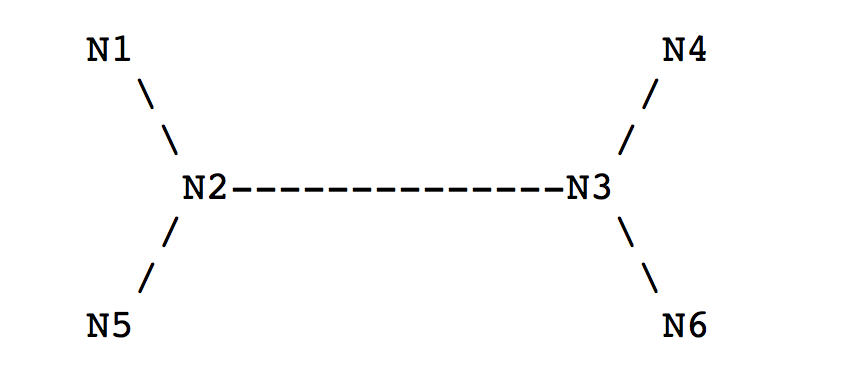
\includegraphics[scale=0.4]{setup.png}
	\caption{We attach TCP agent with FTP as the application, UDP with CBR to this topology.}
	\label{fig:setup}
\end{figure}
We use ns2 to create the topology in Figure \ref{fig:setup}. The setup consists of five different nodes, N1- N5. The link between each pair of nodes is a duplex link with a capacity of 10 Mb.
\subsection{Calculation}
NS2 trace files were used to calculate drop rate, average throughput, average latency and latency over time for combinations of different TCP variants and different queuing algorithms. The trace files were parsed using a python script because of the ease of text parsing with python. We used a python library called the Matplotlib to generate the plots. We use a bash script to automate a series of experiments with varying TCP variant, CBR rate, CBR packet size and queuing algorithms. 
\begin{enumerate}
\item \textbf{Average Throughput:} To calculate the average throughput of the tcp stream, we divide the sum of packet sizes of all TCP packets that reached the destination by the  total time of the tcp flow. 
\item \textbf{Latency:} To calculate latency over time, we recorded the time it took for each packet to get from the source to desination over time. We took the average of latencies over time to get the average latency. 
\item \textbf{Drop Rate:} The ns trace clearly identified the dropped packets. To calculate the drop rate of a flow, we divided the total number of drops by the total number of packets in that flow.
\end{enumerate}
 \subsection{TCP Performance Under Congestion}
This experiment was designed to test the performance of different TCP variants Tahoe, Reno, NewReno and Vegas under various levels of congestion. TCP agent was attached to start at N1 and sink at N4. FTP application was attached to the TCP agent to simulate traffic that is typical of FTP. CBR flow was added to go from N2 to N3 to create congestion in the link between N2 and N3. We varied the CBR rate from 1 Mbps to 10 Mbps to create different levels of congestion. We had the liberty of choosing the packet size to maintain the CBR. To study the effects of varying CBR packet sizes, we also simulated varying packet sizes, 500B to 10,000B, for all four TCP variants. We did not change the default ns2 buffer size of 20 packets.  
 \subsection{Fairness between TCP variants}
This experiment simulated two TCP flows at a time. The variant pairs that were simulated are (1) Tahoe/Tahoe (2) Reno/Reno (3) NewReno/Reno (4) Vegas/Vegas (5) NewReno/Vegas. Like before, to create varying levels of congestion, a CBR flow was added to originate at N2 and end at N3. The first TCP stream originated at added N1 and ended at N4. The second TCP stream originated at N5 and ended at N6. For each pair of the variants, we ran simulations for CBR ranging from 1 Mbps to 10 Mbps. The packet size was 500, constant across all the experiments. We chose this packet size because an average IP packet size is around 600. Accounting for the IP headers, we wanted a smaller packet size for UDP. 
We also started the two competing variants at different times and ran the simulations for a bit longer (15s) to check if fair throughput could be achieved over time if one of the TCP streams was delayed.
 \subsection{Influence of Queuing}
In this experiment, we study the influence of queuing algorithms RED and DropTail on TCP Reno and SACK. The set up for this experiment is the same as experiment 1. We first start the TCP stream, wait till it has passes the slow start phase(at 4s) and then start the CBR flow. We conduct the experiments for two different buffer sizes, 100 and a 300. To compare the performance of RED and DropTail in the TCP variants and the CBR flow, we compare the differences in throughput over time, latency over time and the drop rate between the queuing disciplines. 